%%%%%%%%%%%%%%%%%%%%%%%%%%%%%%%%%%%%%%%%%
% Beamer Presentation
% LaTeX Template
% Version 1.0 (10/11/12)
%
% This template has been downloaded from:
% http://www.LaTeXTemplates.com
%
% License:
% CC BY-NC-SA 3.0 (http://creativecommons.org/licenses/by-nc-sa/3.0/)
%
%%%%%%%%%%%%%%%%%%%%%%%%%%%%%%%%%%%%%%%%%

%----------------------------------------------------------------------------------------
%	PACKAGES AND THEMES
%----------------------------------------------------------------------------------------

\documentclass[9pt]{beamer}
\usepackage{CJK}
\usepackage{ctex}
\usepackage{graphicx}
\usepackage{subfigure}
\usepackage{longtable}
\usepackage{rotating}
\usepackage{multirow}
\usepackage{algorithm}
\usepackage{algorithmic}
\usepackage{mathtools}
\usepackage{animate}
%\usepackage{media9}
%% A LATEX package for embedding interactive Adobe Flash (SWF) and 3D files (Adobe U3D & PRC) as well as video and sound files or streams (FLV, MP4/H.246, MP3) into PDF documents with Adobe Reader-9/X
%compatibility.
\renewcommand{\algorithmicrequire}{\textbf{Input:}}   %Use Input in the format of Algorithm
\renewcommand{\algorithmicensure}{\textbf{Output:}}  %UseOutput in the format of Algorithm
\newcommand{\e}[1]{\ensuremath{\times 10^{#1}}}
%\mode<presentation>{\usetheme{Madrid}}

\mode<presentation> {

% The Beamer class comes with a number of default slide themes
% which change the colors and layouts of slides. Below this is a list
% of all the themes, uncomment each in turn to see what they look like.

%\usetheme{default}
%\usetheme{AnnArbor}
%\usetheme{Antibes}
%\usetheme{Bergen}
%\usetheme{Berkeley}
%\usetheme{Berlin}
%\usetheme{Boadilla}
%\usetheme{CambridgeUS}
%\usetheme{Copenhagen}
%\usetheme{Darmstadt}
%\usetheme{Dresden}
%\usetheme{Frankfurt}
%\usetheme{Goettingen}
%\usetheme{Hannover}
%\usetheme{Ilmenau}
%\usetheme{JuanLesPins}
%\usetheme{Luebeck}
\usetheme{Madrid}
%\usetheme{Malmoe}
%\usetheme{Marburg}
%\usetheme{Montpellier}
%\usetheme{PaloAlto}
%\usetheme{Pittsburgh}
%\usetheme{Rochester}
%\usetheme{Singapore}
%\usetheme{Szeged}
%\usetheme{Warsaw}

% As well as themes, the Beamer class has a number of color themes
% for any slide theme. Uncomment each of these in turn to see how it
% changes the colors of your current slide theme.

%\usecolortheme{albatross}
\usecolortheme{beaver}
%\usecolortheme{beetle}
%\usecolortheme{crane}
%\usecolortheme{dolphin}
%\usecolortheme{dove}
%\usecolortheme{fly}
%\usecolortheme{lily}
%\usecolortheme{orchid}
%\usecolortheme{rose}
%\usecolortheme{seagull}
%\usecolortheme{seahorse}
%\usecolortheme{whale}
%\usecolortheme{wolverine}

%\setbeamertemplate{footline} % To remove the footer line in all slides uncomment this line
%\setbeamertemplate{footline}[page number] % To replace the footer line in all slides with a simple slide count uncomment this line

%\setbeamertemplate{navigation symbols}{} % To remove the navigation symbols from the bottom of all slides uncomment this line
}

\usepackage{graphicx} % Allows including images
\usepackage{booktabs} % Allows the use of \toprule, \midrule and \bottomrule in tables
\begin{document}
\begin{CJK*}{GBK}{kai}
%----------------------------------------------------------------------------------------
%	TITLE PAGE
%----------------------------------------------------------------------------------------

\title[Machine Learning]{K-nearest neighbors} % The short title appears at the bottom of every slide, the full title is only on the title page

%\author{Fuhao Zou(�޸���)}
\author{Fuhao Zou(�޸���)} % Your name
%\logo{%
%   
\includegraphics[scale=.2]{logo.pdf}\hspace*{4.75cm}~%
%   
\includegraphics[scale=.2]{logo.jpg}\hspace*{0.75cm}%
%   }
%\pgfdeclareimage[width=1cm]{hust}{logo.pdf}
%\logo{\pgfuseimage{hust}{\vspace{-10pt}}}
\titlegraphic{
\includegraphics[width=1.3cm]{logo.pdf}}
\institute[IEC, HUST] % Your institution as it will appear on the bottom of every slide, may be shorthand to save space
{
Intelligent and Embedded Computing Lab��\\
                   Huazhong University of Science \& Technology \\ % Your institution for the title page
\medskip
\textit{fuhao\_zou@hust.edu.cn} % Your email address
}

\date{2019��04��09��} % Date, can be changed to a custom date
%====================================================
\frame{\titlepage}

\frame{\frametitle{Table of contents}\tableofcontents}

\AtBeginSection[]
{
\begin{frame}{Table of Contents}
\tableofcontents[currentsection]
\end{frame}
}

%------------------------------------------------
%------------------------------------------------
\section{The k-NN algorithm}
%------------------------------------------------
\subsection{Formal definition of k-NN:}
\begin{frame}
\frametitle{Formal definition of k-NN:}
\begin{block}{Basic idea:}
	In pattern recognition, the k-nearest neighbors algorithm (k-NN) is a non-parametric method used for classification and regression.
\end{block}

\begin{itemize}
	\item Assumption:Similar inputs have similar outputs
	\item Classification rule: For a test input \textbf{x}, assign the most common label amongest its k most similar training inputs
	\item Regression rule: The output is the property value for the object. This value is the average of the values of \textbf{k} nearest neighbors.	
\end{itemize}
\end{frame}
%------------------------------------------------
\begin{frame}
\frametitle{Formal definition of k-NN:}
\begin{block}{Formal definition}
\begin{itemize}
\item Test point: $\mathbf{x}$
\item Denote the set of the $k$ nearest neighbors of $\mathbf{x}$ as $S_\mathbf{x}$. Formally $S_\mathbf{x}$ is defined as $S_\mathbf{x}\subseteq {D}$ s.t. $|S_\mathbf{x}|=k$ and $\forall(\mathbf{x}',y')\in D\backslash S_\mathbf{x}$,
\[\text{dist}(\mathbf{x},\mathbf{x}')\ge\max_{(\mathbf{x}'',y'')\in S_\mathbf{x}} \text{dist}(\mathbf{x},\mathbf{x}''),\]
(i.e. every point in $D$ but \textit{not} in $S_\mathbf{x}$ is at least as far away from $\mathbf{x}$ as the furthest point in $S_\mathbf{x}$).
We can then define the classifier $h()$ as a function returning the most common label in $S_\mathbf{x}$:
\[h(\mathbf{x})=\text{mode}(\{y'':(\mathbf{x}'',y'')\in S_\mathbf{x}\}),\]
where $\text{mode}(\cdot)$ means to select the label of the highest occurrence.
\end{itemize}
\end{block}
\end{frame}

%------------------------------------------------
\subsection{Example}
\begin{frame}
\frametitle{A binary classification example}
\begin{figure}[h]
	\centering
	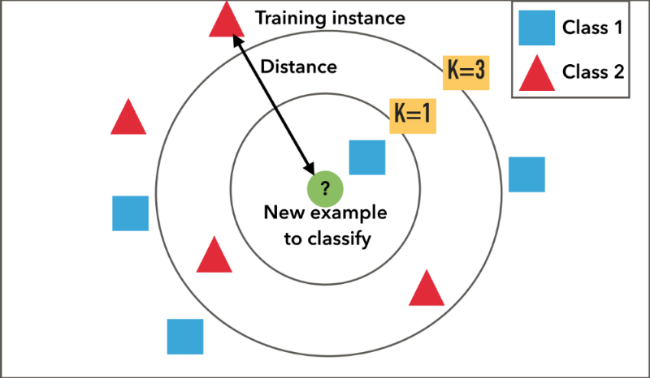
\includegraphics[scale=0.4]{note0}
	\caption{Example of k-NN classification. The test sample (inside circle) should be classified either to the first class of blue squares or to the second class of red triangles. If k = 3 (outside circle) it is assigned to the second class because there are 2 triangles and only 1 square inside the inner circle. If, for example k = 5 it is assigned to the first class (3 squares vs. 2 triangles outside the outer circle).}
\end{figure}
\end{frame}
%------------------------------------------------
\section{Parameter selection}
%------------------------------------------------
\subsection{Distance function}
\begin{frame}
\frametitle{Distance function}
The k-nearest neighbor classifier fundamentally relies on a distance metric. The better that metric reflects label similarity, the better the classified will be. The most common choice is the \textbf{Minkowski distance}
\[\text{dist}(\mathbf{x},\mathbf{z})=\left(\sum_{r=1}^d |x_r-z_r|^p\right)^{1/p}.\]

\begin{block}{Quiz}
	This distance definition is pretty general and contains many well-known distances as special cases. Can you identify the following candidates?
\begin{itemize}
	\item $p=1$
	\item $p=2$
	\item $p \to \infty$
\end{itemize}
\end{block}

\end{frame}
%------------------------------------------------
\subsection{K value}
\begin{frame}
\frametitle{The best K}
\begin{block}{How to choos a K}
	The best choice of \textbf{k} depends upon the data; generally, larger values of \textbf{k} reduces effect of the noise on the classification, but make boundaries between classes less distinct. A good \textbf{k} can be selected by various heuristic techniques (see hyperparameter optimization).
	
	In binary (two class) classification problems, it is helpful to choose \textbf{k} to be an odd number as this avoids tied votes.
	
	Some popular ways of choosing the empirically optimal \textbf{k} includes :
	
	\begin{itemize}
		\item bootstrap method
		\item cross validation
		\item Bayes method
	\end{itemize}
\end{block}
\end{frame}
%%------------------------------------------------


%%------------------------------------------------
\section{Special k-nearest neighbor classifier}
%------------------------------------------------
\subsection{1-nearest neighbor classifier}
\begin{frame}
\frametitle{1-NN classifier}
\begin{block}{1-NN classifier}
	The most intuitive nearest neighbour type classifier is the one nearest neighbour classifier\textbf{(k=1)} that assigns a point \textbf{x} to the class of its closest neighbour in the feature space.
	
	As the size of training data set approaches infinity, the one nearest neighbour classifier guarantees an error rate of no worse than twice the Bayes error rate (the minimum achievable error rate given the distribution of the data).
\end{block}
\end{frame}
%------------------------------------------------
\begin{frame}
\frametitle{1-NN Convergence Proof}
As $n \to \infty$,\textbf{ the $1$-NN error is no more than twice the error of the Bayes Optimal classifier.}
(Similar guarantees hold for $k>1$.)
\begin{figure}
	\begin{minipage}[t]{0.33\linewidth} % ���һ�з�2��ͼ����0.5�����3��ͼ����0.33
		\centering
		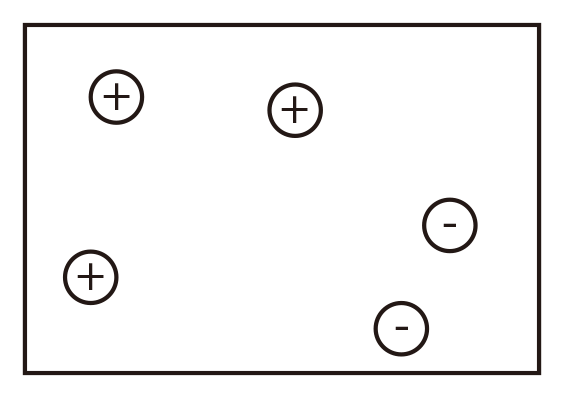
\includegraphics[width= \textwidth]{note2_2_1}
		\caption{$n$ small}
		\label{fig:side:a}
	\end{minipage}%
	\begin{minipage}[t]{0.33\linewidth}
		\centering
		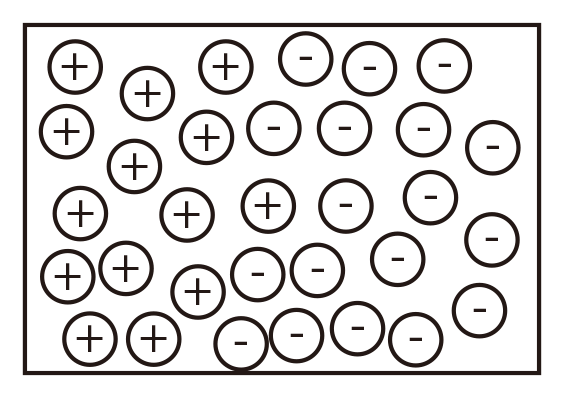
\includegraphics[width= \textwidth]{note2_2_2}
		\caption{$n$ large}
		\label{fig:side:b}
	\end{minipage}
	\begin{minipage}[t]{0.33\linewidth}
	\centering
	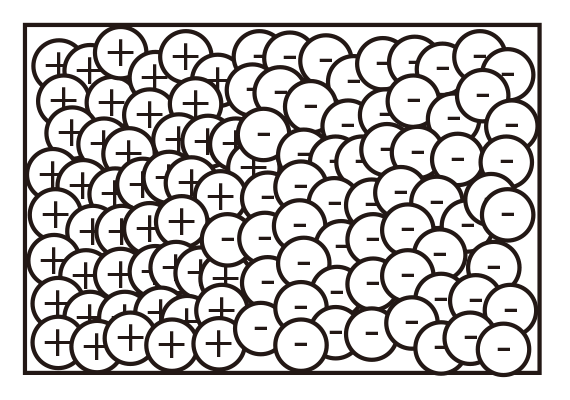
\includegraphics[width= \textwidth]{note2_2_3}
	\caption{$n \to \infty$}
	\label{fig:side:b}
\end{minipage}
\end{figure}
\end{frame}
%------------------------------------------------
\begin{frame}
\frametitle{1-NN Convergence Proof}
Let $\mathbf{x}_\mathrm{NN}$ be the nearest neighbor of our test point $\mathbf{x}_\mathrm{t}$. As $n \to \infty$, $\text{dist}(\mathbf{x}_\mathrm{NN},\mathbf{x}_\mathrm{t}) \to 0$,
i.e. $\mathbf{x}_\mathrm{NN} \to \mathbf{x}_{t}$.
(This means the nearest neighbor is identical to $\mathbf{x}_\mathrm{t}$.)

You return the label of $\mathbf{x}_\mathrm{NN}$.
What is the probability that this is not the label of $\mathbf{x}_\mathrm{t}$?
(This is the probability of drawing two different label of $\mathbf{x}$)
\begin{multline*}
\epsilon_{NN}=\mathrm{P}(y^* | \mathbf{x}_{t})(1-\mathrm{P}(y^* | \mathbf{x}_{NN})) + \mathrm{P}(y^* | \mathbf{x}_{NN})(1-\mathrm{P}(y^* | \mathbf{x}_{t}))\\
\le (1-\mathrm{P}(y^* | \mathbf{x}_{NN}))+(1-\mathrm{P}(y^* | \mathbf{x}_{t}))
= 2(1-\mathrm{P}(y^* | \mathbf{x}_{t}) = 2\epsilon_\mathrm{BayesOpt},
\end{multline*}
where the inequality follows from $\mathrm{P}(y^* | \mathbf{x}_{t})\le 1$ and $\mathrm{P}(y^* | \mathbf{x}_{NN})\le 1$. We also used that $\mathrm{P}(y^* | \mathbf{x}_{t})=\mathrm{P}(y^* | \mathbf{x}_{NN})$.
\end{frame}
%------------------------------------------------
\begin{frame}
\frametitle{1-NN Convergence Proof}
\begin{figure}[h]
	\centering
	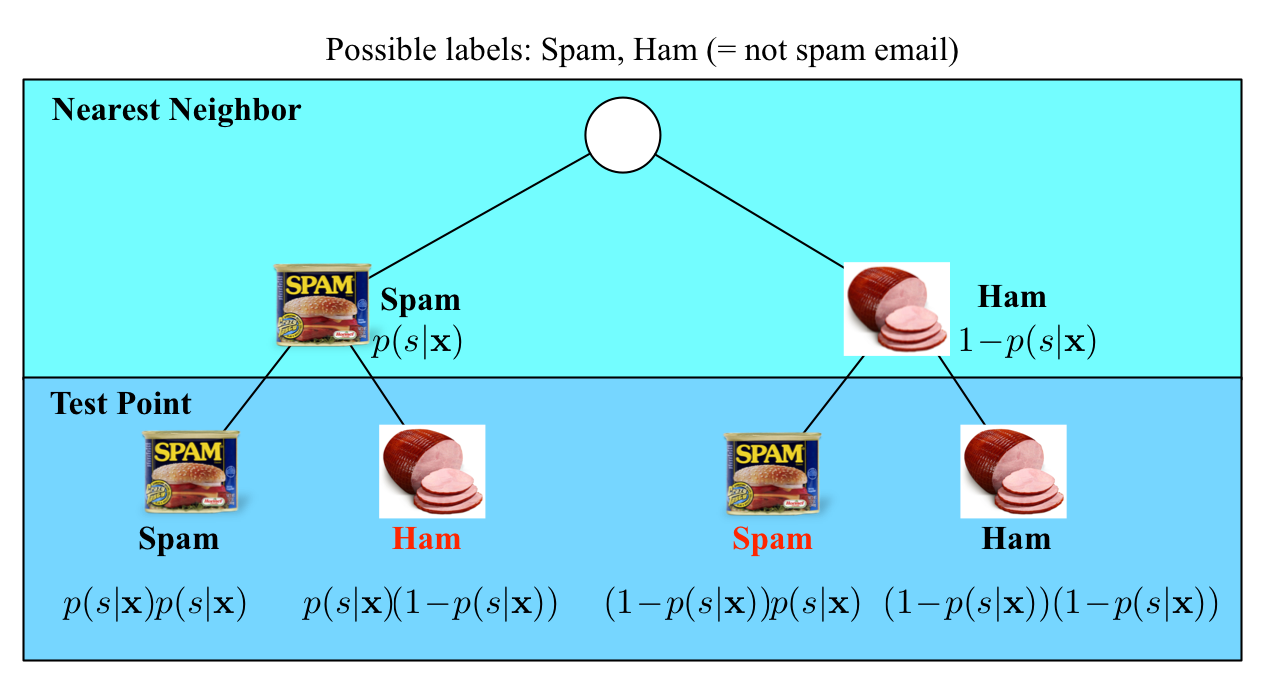
\includegraphics[scale=0.5]{spamtree}
	\caption{In the limit case, the test point and its nearest neighbor are identical.
		There are exactly two cases when a misclassification can occur:
		when the test point and its nearest neighbor have different labels.
		The probability of this happening is the probability of the two red events:
		$(1\!-\!p(s|\mathbf{x}))p(s|\mathbf{x})+p(s|\mathbf{x})(1\!-\!p(s|\mathbf{x}))=2p(s|\mathbf{x})(1-p(s|\mathbf{x}))$ .}
\end{figure}
\end{frame}
%------------------------------------------------
\subsection{*weighted nearest neighbor classifier}
\begin{frame}
\frametitle{*weighted nearest neighbor classifier}
The k-nearest neighbour classifier can be viewed as assigning the \textbf{k} nearest neighbours a weight  \textbf{1/k} and all others 0 weight. This can be generalised to weighted nearest neighbour classifiers. That is, where the ith nearest neighbour is assigned a weight \textbf{$w_{ni}$},with $\sum_{i=1}^{n}{w_{ni}}=1$.An analogous result on the strong consistency of weighted nearest neighbour classifiers also holds.
\end{frame}
%------------------------------------------------
\begin{frame}
\frametitle{*weighted nearest neighbor classifier}
Let${C}_n^{wnn}$ denote the weighted nearest classifier with weights $\{w_{ni}\}_{i=1}^{n}$. Subject to regularity conditions on the class distributions the excess risk has the following asymptotic expansion
$R_R(C_n^{wnn})-R_R(C^{Bayes})=(B_1s_n^2+B_2t_n^2)\{1+o(1)\}$.


for constants $B_1$ and $B_2$ where
$$s_n^2=\sum_{i=1}^{n}w_{ni}^2 \quad and \quad  t_n=n^{-2/d}\sum_{i=1}^{n}w_{ni}\{i^{1+2/d}-(i-1)^{1+2/d}\}$$
The optimal weighting scheme $\{w_{ni}^*\}_{i=1}^{n}$,that balances the two terms in the display above, is given as follows: set $k^*=\lfloor{Bn^{\frac{4}{d+4}}}\rfloor$
$$w_{ni}^*=\frac{1}{k^*}[1+\frac{d}{2}-\frac{d}{2k^{*2/d}}\{i^{1+2/d}-(i-1)^{1+2/d}\}] \quad for\quad i=1,2,...k^* \quad and $$
$$w_{ni}^*=0 \quad for \quad i=k^*+1,...,n$$
With optimal weights the dominant term in the asymptotic expansion of the excess risk is $O(n^{-{\frac{4}{d+4}}})$. Similar results are true when using a bagged nearest neighbour classifier.
\end{frame}

%%------------------------------------------------
\section{Curse of Dimensionality}
%------------------------------------------------
\subsection{Distances between points}
\begin{frame}
\frametitle{Distances between points}
Formally, imagine the unit cube $[0,1]^d$.  All training data is sampled \textit{uniformly}
within this cube, i.e. $\forall i, x_i\in[0,1]^d$, and we are considering the $k=10$ nearest neighbors of such a test point.
\begin{figure}[h]
	\centering
	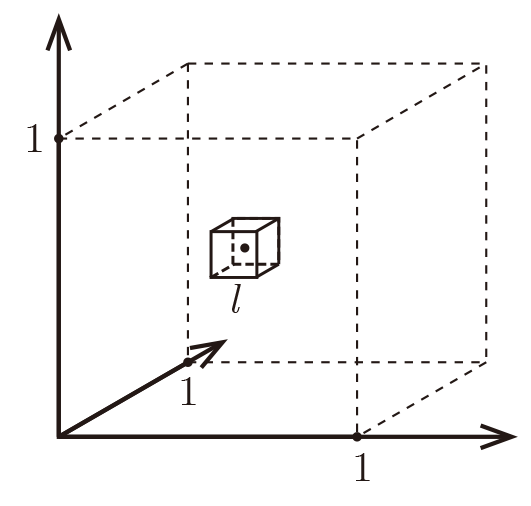
\includegraphics[scale=0.8]{note2_3}
\end{figure}
Let $\ell$ be the edge length of the smallest hyper-cube that contains all $k$-nearest neighbor of a test point.
Then $\ell^d\approx\frac{k}{n}$ and $\ell\approx\left(\frac{k}{n}\right)^{1/d}$.

\end{frame}
%------------------------------------------------
\begin{frame}
\frametitle{Distances between points}
\begin{figure}[h]
	\centering
	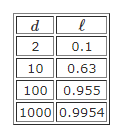
\includegraphics[scale=0.5]{note2_3_table}
\end{figure}
So as $d\gg 0$ almost the entire space is needed to find the $10$-NN. This breaks down the $k$-NN assumptions, because the $k$-NN are not particularly closer (and therefore more similar) than any other data points in the training set. Why would the test point share the label with those $k$-nearest neighbors, if they are not actually similar to it?

\end{frame}
%------------------------------------------------
\begin{frame}
\frametitle{Distances between points}
\begin{figure}[h]
	\centering
	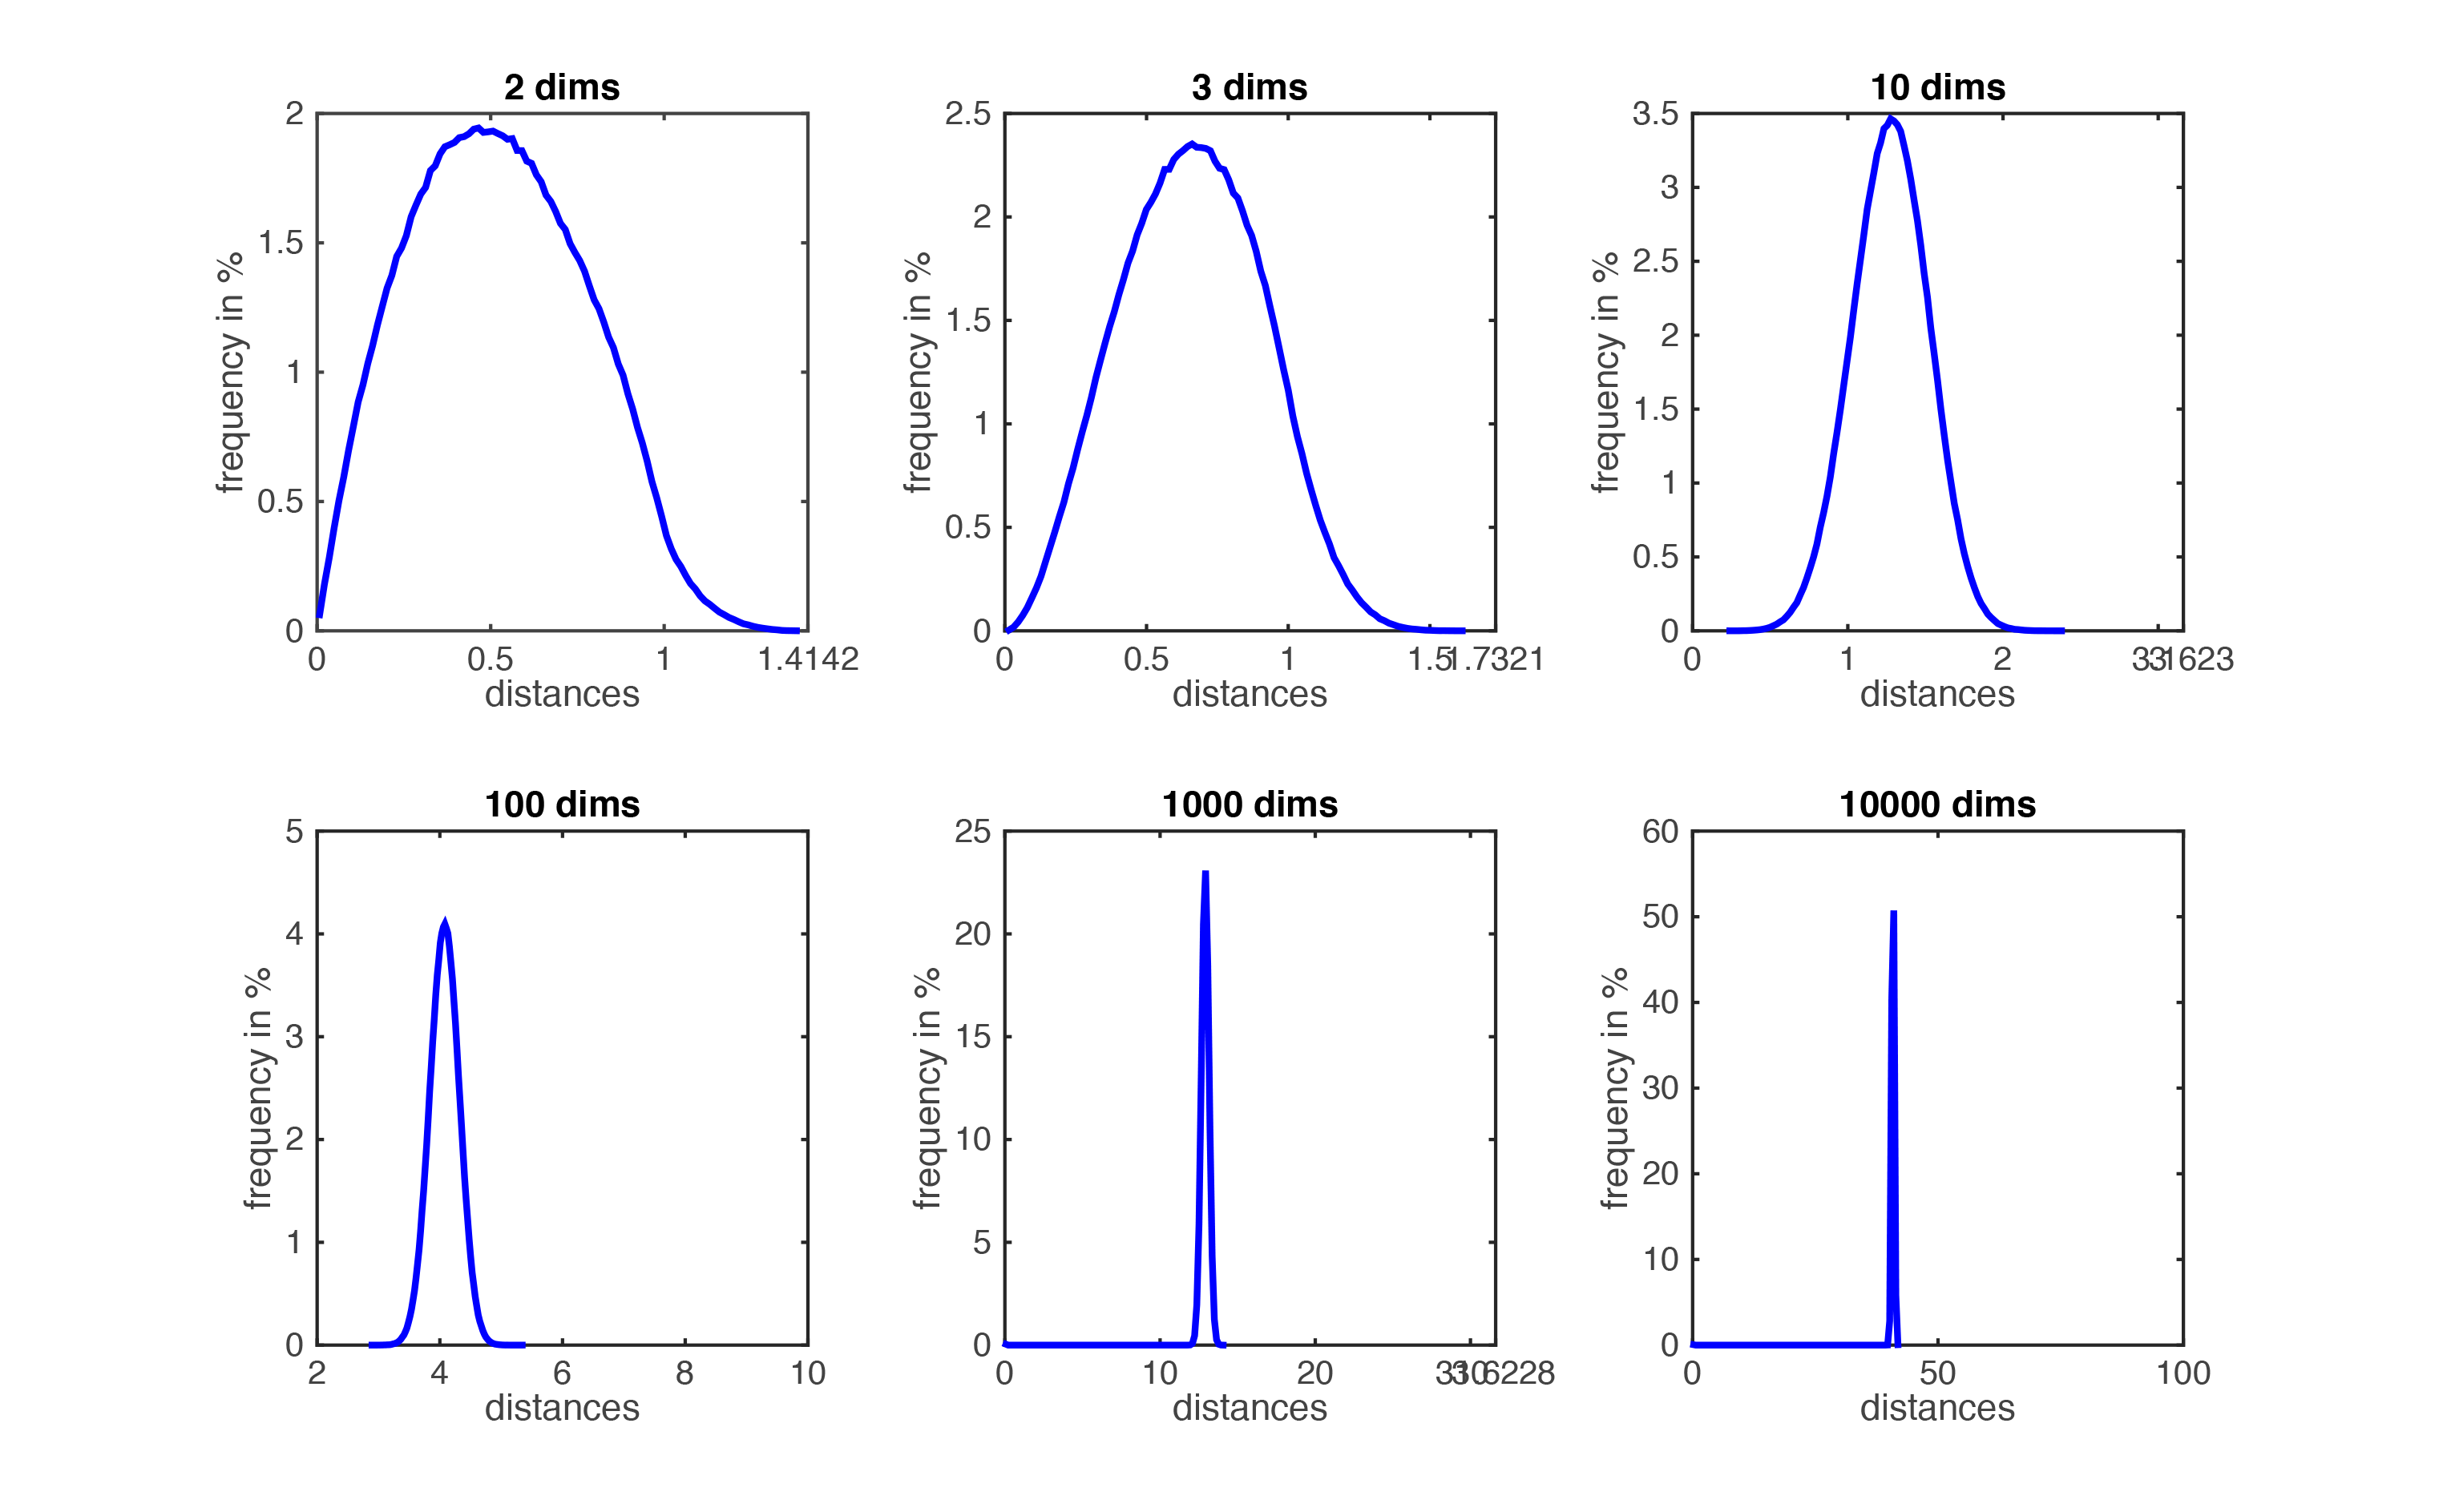
\includegraphics[scale=0.4]{cursefigure}
	\caption{Figure demonstrating ``the curse of dimensionality''. The histogram plots show the distributions of all pairwise distances between randomly distributed points within $d$-dimensional unit squares.  As the number of dimensions $d$ grows, all distances concentrate within a very small range .}
\end{figure}
\end{frame}
%------------------------------------------------
\subsection{Distances to hyperplanes}
\begin{frame}
\frametitle{Distances to hyperplanes}
\begin{block}{Thinking}
	The distance between two randomly drawn data points increases drastically with their dimensionality. How about the distance to a hyperplane?
\end{block}
\begin{figure}[h]
	\centering
	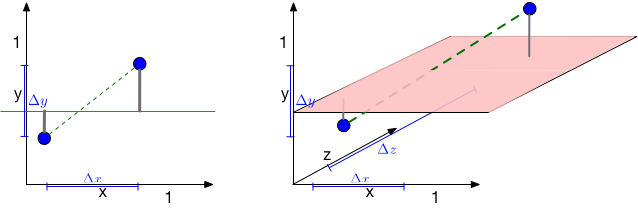
\includegraphics[scale=0.5]{cursePointHyperplane}
	\caption{The curse of dimensionality has different effects on distances between two points and distances between points and hyperplanes .}
\end{figure}
\end{frame}

%%------------------------------------------------
\section{How to solve the curse of dimensionality}
%------------------------------------------------
\subsection{Dimension reduction}
\begin{frame}
\frametitle{Dimension reduction}
\begin{block}{Dimension reduction}
	 For high-dimensional data (e.g., with number of dimensions more than 10) dimension reduction is usually performed prior to applying the k-NN algorithm in order to avoid the effects of the curse of dimensionality.
	

	Feature extraction and dimension reduction can be combined in one step using principal component analysis (\textbf{PCA}), linear discriminant analysis (\textbf{LDA}), or canonical correlation analysis (\textbf{CCA}) techniques as a pre-processing step, followed by \textbf{clustering} by k-NN on feature vectors in reduced-dimension space. In machine learning this process is also called \textbf{low-dimensional embedding}.		
\end{block}
\end{frame}
%------------------------------------------------
\subsection{Data reduction}
\begin{frame}
\frametitle{Data reduction}
\begin{block}{Data reduction}
	Data reduction is one of the most important problems for work with huge data sets. Usually, only some of the data points are needed for accurate classification. Those data are called the \textbf{prototypes} and can be found as follows:
	\begin{enumerate}[1]
		\item Select the \textbf{class-outliers}, that is, training data that are classified incorrectly by k-NN (for a given k)
		\item Separate the rest of the data into two sets: (i) the prototypes that are used for the classification decisions and (ii) the absorbed points that can be correctly classified by k-NN using prototypes. The absorbed points can then be removed from the training set.
	\end{enumerate}
\end{block}

\end{frame}
%------------------------------------------------
\begin{frame}
\frametitle{Selection of class-outliers}
A training example surrounded by examples of other classes is called a \textbf{class outlier}. Causes of class outliers include:
\begin{itemize}
	\item random error
	\item insufficient training examples of this class (an isolated example appears instead of a cluster)
	\item missing important features (the classes are separated in other dimensions which we do not know)
	\item too many training examples of other classes (unbalanced classes) that create a "hostile" background for the given small class
\end{itemize}

Class outliers with k-NN produce noise. They can be detected and separated for future analysis. Given two natural numbers, \textbf{$k \textgreater r \textgreater 0$}, a training example is called a \textbf{(k,r)}NN class-outlier if its \textbf{k} nearest neighbors include more than \textbf{r} examples of other classes.
\end{frame}

%%------------------------------------------------
\section{k-NN summary}
\subsection{Quick summary of k-NN}
\begin{frame}
\frametitle{Quick summary of k-NN}
\begin{itemize}
	\item k-NN is a simple and effective classifier if distances reliably reflect a semantically meaningful notion of the dissimilarity. (It becomes truly competitive through metric learning)
	\item As $n \to \infty$, k-NN becomes provably very accurate, but also very slow.
	\item As $d \gg 0$, points drawn from a probability distribution stop being similar to each other, and the k-NN assumption breaks down.
	\item k-NN stores the entire training dataset which it uses as its representation.
	\item k-NN does not learn any model.
	\item k-NN makes predictions just-in-time by calculating the similarity between an input sample and each training instance.
\end{itemize}
\end{frame}
%------------------------------------------------
\subsection{Pros and cons of k-NN}
\begin{frame}
\frametitle{Pros and cons of k-NN}
\textcolor[rgb]{0.00,0.07,1.00}{\textbf{Some pros and cons of k-NN:}}
\begin{block}{Pros}
	\begin{itemize}
		\item No assumptions about data �� useful, for example, for nonlinear data
		\item Simple algorithm �� to explain and understand/interpret
		\item High accuracy (relatively) �� it is pretty high but not competitive in comparison to better supervised learning models
		\item Versatile �� useful for classification or regression
	\end{itemize}
\end{block}
\begin{block}{Cons}
	\begin{itemize}
		\item Computationally expensive �� because the algorithm stores all of the training data
		\item High memory requirement
		\item Stores all (or almost all) of the training data
		\item Prediction stage might be slow (with big N)
		\item Sensitive to irrelevant features and the scale of the data
	\end{itemize}	
\end{block}

\end{frame}
%%------------------------------------------------
%\section{Reference}
%------------------------------------------------
%\begin{frame}
%\frametitle{Reference}
%\begin{thebibliography}{4}
%\bibitem{LS-SPH} F. Zou, C. Liu, H. Ling, H. Feng, L. Yan, and D. Li, "Least square regularized spectral hashing for similarity search," Signal Processing, vol. 93, pp. 2265-2273, 2013. (SCI,EI)
%\bibitem{KMFH} F. Zou, Y. Chen, J. Song, K. Zhou, Y. Yang, and N. Sebe, "Compact image fingerprint via multiple kernel hashing," IEEE Transactions on Multimedia, vol. 17, pp. 1006-1018, 2015. (SCI,EI)
%\bibitem{KNPH} C. Liu, H. Ling, F. Zou, L. Yan, Y. Wang, H. Feng, et al., "Kernelized neighborhood preserving hashing for social-network-oriented digital fingerprints," IEEE Transactions on Information Forensics and Security, vol. 9, pp. 2232-2247, 2014. (SCI,EI)
%\bibitem{DTSH} Liu, Yu; Song, Jingkuan; Zhou, Ke; Yan, Lingyu; Liu, Li; Zou, Fuhao; Shao, Ling, "Deep Self-taught Hashing for Image Retrieval," IEEE Transactions on Cybernetics, May 3, 2018. (SCI,EI)
%\bibitem{DeepFace} Fuhao Zou, Fan Yang, Wei Chen,Kai Lia, Jingkuan Song, Jingcai Chen, Hefei Ling, "Fast Large Scale Deep Face Search," Pattern Recognition Letters, Januray 3, 2019. (SCI,EI)
%\end{thebibliography}
%\end{frame}
%------------------------------------------------
\begin{frame}
\Huge{\centerline{The End}}
\end{frame}
\end{CJK*}
\end{document}
%\end{document}
